\documentclass{beamer}
%\documentclass[handout]{beamer}
%\setbeameroption{show notes}

% Think backwards: what do you want people to remember from your talk?
% Don’t say everything.
% Simplify.

\setbeamertemplate{navigation symbols}{}%remove navigation symbols
\setbeamercolor{normal text}{fg=white,bg=black!90}
\setbeamercolor{structure}{fg=white}
\setbeamercolor{alerted text}{fg=red!85!black}
\setbeamercolor{item projected}{use=item,fg=black,bg=item.fg!35}
\setbeamercolor*{palette primary}{use=structure,fg=structure.fg}
\setbeamercolor*{palette secondary}{use=structure,fg=structure.fg!95!black}
\setbeamercolor*{palette tertiary}{use=structure,fg=structure.fg!90!black}
\setbeamercolor*{palette quaternary}{use=structure,fg=structure.fg!95!black,bg=black!80}
\setbeamercolor*{frametitle}{fg=blue!40}
\setbeamercolor*{framesubtitle}{fg=blue!30}
\setbeamercolor*{block title}{parent=structure,bg=black!60}
\setbeamercolor*{block body}{fg=black,bg=black!10}
\setbeamercolor*{block title alerted}{parent=alerted text,bg=black!15}
\setbeamercolor*{block title example}{parent=example text,bg=black!15}

\usepackage{listings}
\usepackage[english]{babel}
\usepackage[utf8]{inputenc}
\usepackage{amsmath}
\usepackage{graphicx}
\usepackage{fontenc}

\usepackage{tikz}
\usetikzlibrary{fadings}

\title[{Nopol: Repairing Bugs in Conditional Expressions}]{Nopol:~Repairing~Bugs~in~Conditional~Expressions}
\author[Favio DeMarco]{Favio~DeMarco}
\institute[U.B.A. - INRIA]{Universidad de Buenos Aires - INRIA}
\date{\today}
\subject{Computational Sciences}

\begin{document}

  \frame
  {
\begin{quote}
    Take nothing on its looks; take everything on evidence. There's no better rule.
\end{quote}    
– Charles Dickens, ``Great Expectations.''
  }

\frame
  {
  \begin{center}
  
\includegraphics[width=7em]{logofcen}
  \end{center}
    \titlepage
  }

\begin{frame}  
\frametitle{Bugs}
\begin{quotation}
The difference between the right word and the almost right word is the difference between lightning and a lightning bug.
\end{quotation}
-- Mark Twain
\end{frame}
 
  
\begin{frame}[fragile]
\frametitle{What are conditional bugs?}
\begin{lstlisting}[escapeinside=\[\]]
[\textbf{boolean expression}] ? someValue : someOtherValue;
\end{lstlisting}

\begin{lstlisting}[escapeinside=\[\]]
if ([\textbf{boolean expression}]) {
...
\end{lstlisting}
\end{frame}

\begin{frame}[fragile]
\frametitle{Change of If Condition Expression (IF-CC)}
Kai Pan et al.:
\begin{quotation}
This bug fix change fixes the bug by changing the condition expression of an if
condition. The previous code has a bug in the if condition logic.
\end{quotation}

\vspace{1em}

\begin{lstlisting}
- if (getView().countSelected() == 0) {
+ if (getView().countSelected() <= 1) {
\end{lstlisting}
\end{frame}
  
\begin{frame}[fragile]
\frametitle{What are conditional bugs?}
\framesubtitle{Commons Math - MathUtils class}
    
\begin{lstlisting}[escapeinside=\[\]]
411: public static int gcd(int u, int v) {
412:   if ([\textbf{u * v == 0}]) {
413:     return (Math.abs(u) + Math.abs(v));
414:   }
...
\end{lstlisting}

\vspace{2em}

\centering What about \texttt{u=0x00110000} and  \texttt{v=0x01100000}?

\end{frame}

\begin{frame}
\frametitle{Problem I}
\framesubtitle{How to find the bug?}
How do we know something is \textit{wrong}?
\end{frame}

\begin{frame}
\frametitle{Problem I}
\framesubtitle{How to find the bug?}
Some kind of specification:
\begin{itemize}
 \item Model
 \item Contracts
 \item \textbf{Unit tests}
 \item ...
\end{itemize}
\end{frame}

\begin{frame}[fragile]
    \frametitle{Case study}
      \framesubtitle{Commons Math}
At least one failing test:
      
      \begin{lstlisting}[escapeinside=\[\]]
assertEquals([\textbf{3 * (1$<<$15)}]
       , gcd(3 * (1<<20), 9 * (1<<15)));
	\end{lstlisting}
\end{frame}

\begin{frame}
\frametitle{No-Pol input}
\begin{itemize}
 \item Java source code.
 \item Unit tests with at least one failing test case.
 \item Dependencies (\textit{classpath}).
\end{itemize}
\end{frame}

\begin{frame}
\frametitle{No-Pol output}
Patched Java source file.
\end{frame}


\frame
{
    \frametitle{Overview}
    \framesubtitle{Trial and error}
  \begin{center}
  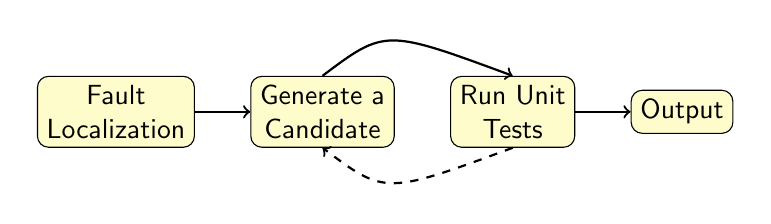
\begin{tikzpicture}[
  font=\sffamily,
  every matrix/.style={ampersand replacement=\&,column sep=2em,row sep=2em},
  box/.style={draw,rounded corners,fill=yellow!20},
  flow/.style={->, thick},
  fail/.style={->, thick, dashed},
  every node/.style={align=center}]
  
% Position the nodes using a matrix layout
\matrix{
      \node[box] (faultLocalization) {Fault \\ Localization};
      \& \node[box] (generateCandidate) {Generate a \\ Candidate};
      \& \node[box] (test) {Run Unit \\ Tests};
      \& \node[box] (output) {Output};
      \\
  };

% Draw the arrows between the nodes and label them.
\draw [flow] (faultLocalization) -- (generateCandidate);
\draw [flow] (generateCandidate.north) .. controls (up:3em) .. (test.north);
\draw [flow] (test) -- (output);
\draw [fail] (test.south) .. controls (down:3em) .. (generateCandidate.south);


% \draw [fail] (oracleInquisition.south) .. controls (down:.5em) and (left:8em) .. (oracleInquisition.west);
% \draw [fail] (collectionOfTestExecutionData) .. controls (down:2em) and (left:9em) .. (oracleInquisition.west);
% \draw [fail] (smtSolving.north) .. controls (down:2em) and (left:10em) .. (oracleInquisition.west);
\end{tikzpicture}

  \end{center}
}


\begin{frame}[fragile]
    \frametitle{Fault Localization (statement ranking)}
      \framesubtitle{GZoltar - Ochiai coefficient}
The suspiciousness $s_j$ of a statement $j$ depends on:
\begin{itemize}
 \item The number of \textbf{failing} test cases \textbf{executing} statement $j$ 
 \item The number of \textbf{failing} test cases \textbf{not executing} statement $j$
 \item The number of \textbf{successful} tests \textbf{executing} statement $j$
\end{itemize}
\end{frame}


\begin{frame}[fragile]
\frametitle{Fault Localization (statement ranking)}
\framesubtitle{GZoltar - Ochiai coefficient}
\begin{verbatim}
MathUtils:413 - Suspiciousness: 0.23570226039551587
MathUtils:431 - Suspiciousness: 0.1543033499620919
\end{verbatim}
...
\begin{verbatim}
MathUtils:460 - Suspiciousness: 0.11322770341445956
MathUtils:412 - Suspiciousness: 0.11180339887498948
\end{verbatim}
...
\end{frame}


\begin{frame}[fragile]
\frametitle{Fault Localization (statement ranking)}
\framesubtitle{GZoltar - Ochiai coefficient}
\begin{verbatim}
...
MathUtils:460 - Suspiciousness: 0.11322770341445956
MathUtils:412 - Suspiciousness: 0.11180339887498948
...
\end{verbatim}

\begin{lstlisting}[escapeinside=\[\]]
411: public static int gcd(int u, int v) {
412:   if ([\textbf{u * v == 0}]) {
413:     return (Math.abs(u) + Math.abs(v));
414:   }
\end{lstlisting}
\end{frame}


\frame
{
  \frametitle{Oracle Inquisition}
  \framesubtitle{For Location \texttt{x}}
  \begin{center}
  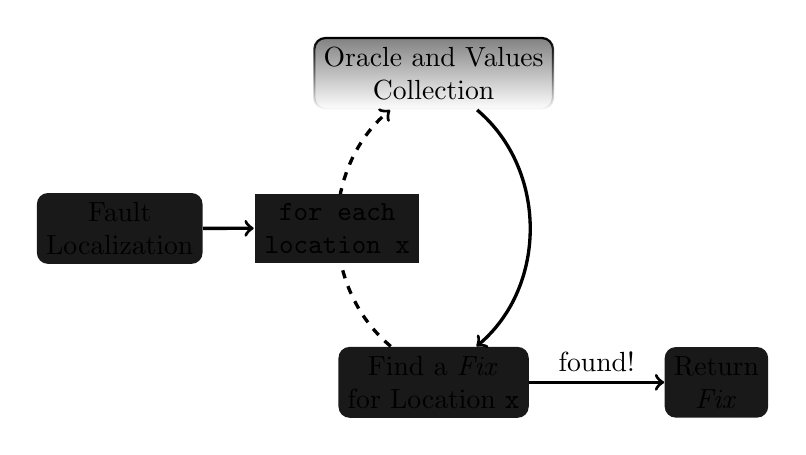
\begin{tikzpicture}[
  every matrix/.style={ampersand replacement=\&,column sep=4em,row sep=3em},
  box/.style={rounded corners,fill=gray,path fading=south, draw, thick},
  shadedbox/.style={rounded corners,fill=black!90},
  flow/.style={->, very thick},
  fail/.style={->, very thick, dashed},
  every node/.style={align=center}]
  
% Position the nodes using a matrix layout
\matrix{

      \& \node[box] (test) {Oracle and Values \\ Collection};
      \& \\
      \node[shadedbox] (faultLocalization) {Fault \\ Localization};
      \& \\
      \& \node[shadedbox] (generateCandidate) {Find a \textit{Fix} \\ for Location \texttt{x}};
      \& \node[shadedbox] (output) {Return \\ \textit{Fix}};
      \\
  };

% Draw the arrows between the nodes and label them.
\draw [flow] (test) to[bend left=50] (generateCandidate);
\draw [flow] (generateCandidate) to node[above] {found!} (output);
\draw [fail] (generateCandidate) to[bend left=50] node[font=\ttfamily, fill=black!90] (statement) {for each \\ location x} (test);
\draw [flow] (faultLocalization) -- (statement.west);

\end{tikzpicture}

  \end{center}
}

\frame
{
  \frametitle{Oracle Inquisition}
  \framesubtitle{For Location \texttt{x}}
  \begin{center}
  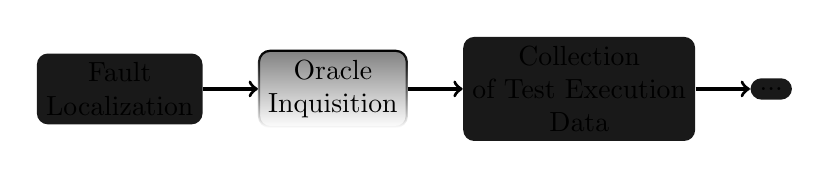
\begin{tikzpicture}[
  every matrix/.style={ampersand replacement=\&,column sep=2em,row sep=2em},
  box/.style={rounded corners,fill=gray,path fading=south, draw, thick},
  shadedbox/.style={rounded corners,fill=black!90},
  flow/.style={->, very thick},
  fail/.style={->, thick, dashed},
  every node/.style={align=center}]
  
% Position the nodes using a matrix layout
\matrix{
    \node[shadedbox] (faultLocalization) {Fault \\ Localization};
    \& \node[box] (oracleInquisition) {Oracle \\ Inquisition};
    \& \node[shadedbox] (collectionOfTestExecutionData) {Collection \\ of Test Execution \\ Data};
    \& \node[shadedbox] (empty) {...};
    \\
  };

% Draw the arrows between the nodes and label them.
\draw [flow] (faultLocalization) -- (oracleInquisition);
\draw [flow] (oracleInquisition) -- (collectionOfTestExecutionData);
\draw [flow] (collectionOfTestExecutionData) -- (empty);

\end{tikzpicture}

  \end{center}
}

\begin{frame}[fragile]
  \frametitle{Generating a candidate}
  \framesubtitle{Oracle-Guided Component-Based Program Synthesis:}
  Components and line numbers:
\begin{verbatim}
0 true
1 false
2 0
3 1
4 u
5 v
...
O1 I1_1 < I1_2
O2 I2_1 <= I2_2
O3 I3_1 + I3_2
...
ON IN_1 ? IN_2 : IN_3
\end{verbatim}
\end{frame}

\begin{frame}[fragile]
  \frametitle{Generating a candidate}
  \framesubtitle{Example}
  Components:
\begin{verbatim}
0 I
O1 := f1(I1);
O2 := f2(I2_1, I2_2);
\end{verbatim}
I want to codify:
\begin{verbatim}
f(I) = f1(f2(I, I));
\end{verbatim}
\end{frame}

\begin{frame}[fragile]
  \frametitle{Generating a candidate}
  \framesubtitle{Example}
\begin{columns}
\column{.5\textwidth}
  Components:
\begin{verbatim}
0 I
O1 := f1(I1);
O2 := f2(I2_1, I2_2);
\end{verbatim}
I want to codify:
\begin{verbatim}
f(I) = f1(f2(I, I));
\end{verbatim}
\column{.5\textwidth}
A solution:
\begin{verbatim}
0 I
1 := f2(0, 0);
2 := f1(1);
\end{verbatim}
Line coded:
\begin{verbatim}
I1 = 1    O1 = 2
I2_1 = 0  O2 = 1
I2_2 = 0  O  = 2
\end{verbatim}
\end{columns}
\end{frame}


\frame
{
  \frametitle{Generating a candidate}
  \framesubtitle{Oracle-Guided Component-Based Program Synthesis}
\begin{equation*}
\phi_{func}(L, I, O) = \exists P, R \psi_{wfp}(L, I, P, R) \wedge \psi_{lib}(P, R) \wedge \psi_{conn}(L, I, O, P, R)
\end{equation*}
}


\frame
{
  \frametitle{Generating a candidate}
  \framesubtitle{Oracle-Guided Component-Based Program Synthesis}
\begin{equation*}
\psi_{wfp}(L, I, P, R) = \bigwedge_{x \in P} (0 \leq l_x < M) \wedge \bigwedge_{x \in R} (|I| \leq l_x < M)
\end{equation*}
\begin{equation*}
\wedge \psi_{cons}(L) \wedge \psi_{acyc}(L)
\end{equation*}
}

\frame
{
  \frametitle{Generating a candidate}
  \framesubtitle{Oracle-Guided Component-Based Program Synthesis}
\begin{equation*}
\psi_{lib}(P, R) = \left( \bigwedge^N_{i=1} \phi_i(I_i, O_i) \right)
\end{equation*}

\begin{equation*}
\psi_{conn}(L, I, O, P, R) = \bigwedge_{x, y \in P \cup R \cup I \cup \{O\}} (l_x = l_y \Rightarrow x = y)
\end{equation*}
}

  \frame
  {
    \frametitle{Problems}
\begin{itemize}
\item Can't automate the testing process.
\item It's not easy to find candidates.
\end{itemize}    
  }

  \frame
  {
    \frametitle{Problems}
    \framesubtitle{Test quality}
   \begin{quote}
    Quality is free, but only to those who are willing to pay heavily for it.
   \end{quote}
    Tom DeMarco, Peopleware   
  }
  
  \frame
  {
    \frametitle{Limitations}
    \framesubtitle{Test quality}
\begin{itemize}
\item Only 1 set of input values.
\item Branch coverage.
\item A \textit{removed} precondition can generate an infinite loop.
\item Tests that exercise both branches.
\item Generates \textit{a} fix not \textbf{THE} fix.
\end{itemize}        
  }

  \frame
  {  
    \frametitle{Contributions}
      \framesubtitle{Process}
\begin{itemize}
\item Statement ranking (GZoltar)  $\rightarrow$
\item Ad hoc code manipulation and values capturing $\rightarrow$
\item Repair Constraint  $\rightarrow$
\item Program Synthesis (OGCBPS\footnote{Oracle-Guided Component-Based Program Synthesis} -paper-)
\end{itemize}
}


  \frame
  {
    \frametitle{Experimental methodology}
    Seeded and wild bugs.
  }
  
  \frame
  {
    \frametitle{Evaluation / Validation}
    Generated patches vs. reality.
  }
  
  \frame
  {
    \frametitle{Perspectives}
    
  }
  
  \frame
  {
    \frametitle{Conclusion}
    
  }

  \frame
  {
    \frametitle{Contribution}
    
  }
  
 \begin{frame}[fragile]
    \frametitle{Case study}
      \framesubtitle{Commons Math - MathUtils class}
\begin{lstlisting}[escapeinside=\[\]]
411: public static int gcd(int u, int v) {
412:   if ([\textbf{u * v == 0}]) {
413:     return (Math.abs(u) + Math.abs(v));
414:   }
...
\end{lstlisting}
\end{frame}

 \begin{frame}[fragile]
    \frametitle{Case study}
      \framesubtitle{Commons Math}
        \begin{lstlisting}[escapeinside=\[\]]
assertEquals([\textbf{3 * (1$<<$15)}]
        , gcd(3 * (1<<20), 9 * (1<<15)));
	\end{lstlisting}
\end{frame}

 \begin{frame}[fragile]
    \frametitle{Case study}
      \framesubtitle{Statement ranking (GZoltar)}
\begin{verbatim}
MathUtils:413 Suspiciousness 0.23570226039551587
MathUtils:431 Suspiciousness 0.1543033499620919
\end{verbatim}
...
\begin{verbatim}
MathUtils:460 Suspiciousness 0.11322770341445956
MathUtils:412 Suspiciousness 0.11180339887498948
\end{verbatim}
\end{frame}

 \begin{frame}[fragile]
    \frametitle{Case study}
      \framesubtitle{Ad hoc code manipulation and values capturing (OGCBPS -paper-)}
\begin{lstlisting}[escapeinside=\[\]]
411: public static int gcd(int u, int v) {
412:   if ([\textbf{true}]) {
413:     return (Math.abs(u) + Math.abs(v));
414:   }
...
\end{lstlisting}
\end{frame}

 \begin{frame}[fragile]
    \frametitle{What are conditional bugs?}
    \framesubtitle{Commons Math - MathUtils class}
        \begin{lstlisting}[escapeinside=\[\]]
public static int gcd(int u, int v) {
    if ([\textbf{(u == 0) $||$ (v == 0)}]) {
        return (Math.abs(u) + Math.abs(v));
    }
    // ...
}
	\end{lstlisting}
\end{frame}

\end{document}
